% !TeX root = ../NotesOnLQG.tex

\chapter{协变圈量子引力——spinfoam 模型}

	本章介绍 spinfoam 模型(又称协变圈量子引力)。这种模型给出了定义在复形上的振幅,被普遍认为是广义相对论的路径积分量子化及给出圈量子引力中的物理内积的一个候选理论。

	自从 \cite{Misner1957} 以来,物理学家不断地考虑量子引力的路径积分表述的可行性。在 QGD 中考虑路径积分,给定 $D$ 是夹在类空超曲面 $\Sigma,\Sigma'$ 之间的时空区域,$\Sigma$ 上的黎曼度规等价类 $[h]$ 和 $\Sigma'$ 上的黎曼度规 $h'$ 的微分同胚等价类 $[h']$ 之间的跃迁振幅形式地写为
	\begin{equation}
		W([h],[h']) = \ip{[h]}{[h']} = \int_{\superspace{D}} \mathcal{D}[g] \e{\ii S(g)},\label{eq-GR_path_integral}
	\end{equation}
	其中 $\superspace{D}$ 是之前定义过的超空间,即度规微分同胚等价类的集合。$S(g) = S_{\text{EH}}(g) + S_{\text{boundary term}}(g)$。根据量子力学,$W([h],[h'])$ 在固定 $[h]$ 或 $[h']$ 时作为另一个的函数,将是 Wheeler DeWitt 方程的解,即 QGD 的一个物理态。然而,该式的定义十分困难:$\superspace{D}$ 上的积分测度尚未有定义,并且由于曾经提到的 QGD 的希尔伯特空间难以明确定义,边界态 $\ket{[h]}$ 也没有清楚的定义。

	这些困难在用 LQG 代替 QGD 后有了新的可能性。在 LQG 中,已经定义好了代表3维几何的 $\HDiff$,spin-network state 代替了 $[h]$,因而边界态的定义没有问题。相应的 $[g]$ 则由 spinfoam 代替。1961 年 Tullio Regge 基于每一个洛伦兹流形都可单纯剖分的事实提出了 Regge calculus\cite{Regge1961}。
	Regge 将时空流形进行单纯剖分,用单复形逼近时空,将曲率离散化为不足角,则所有边长构成了位型变量,爱因斯坦-希尔伯特作用量被改写为 Regge 作用量。注意到对单复形可定义对偶复形,它与边界交于一些点、线,即诱导一个边界图,于是边界图上恰好可以定义 spin-network state 来表示边界态,于是 spinfoam 的构想是对时空三角剖分,边界图上标记自旋量子数和 intertwiner,在内部的复形上也标记自旋量子数和 intertwiner,称为 spinfoam,并用对 spinfoam 求和来定义对 $[g]$ 求和。最终,该模型被证明在半经典极限下可以给出 Regge 作用量,即广义相对论的离散版本。

	\section{单复形的对偶复形}

		先回顾一下代数拓扑或几何中 \emph{$n$-单形}($n$-simplex)及 \emph{单复形}(simplicial complex)的定义:$n$-单形是几何无关的 $n+1$ 个点的凸包,例如 $1$-单形是线段,$2$-单形是三角形,$3$-单形是四面体,$n$ 称为单形的维数。每个单形上可赋予两个定向。$n$-单形 $s$ 中去掉 $m$ 个顶点后张成的单形称为 $s$ 的 $n-m$ 维面。单复形 $\complex{K} = \left\{ s_1, \cdots, s_N \right\}$ 是一组单形的集合,满足每个单形 $s\in \complex{K}$ 的所有面也都属于 $\complex{K}$,且 $\complex{K}$ 中的每两个单形要么不交,要么交于一个公共面。$\complex{K}$ 中的单形维数最大值称为 $\complex{K}$ 的维数,则 $n$ 维单复形 $\complex{K}$ 对应的 $\abs{\complex{K}} \definedby \bigcup_{s\in \complex{K}} s$ 是一个 $n$ 维多面体。
		% \begin{Definition}
		% 	\begin{enumerate}
		% 		\item 给定欧式空间中几何独立的 $n+1$ 个点 $\left\{ x_i \right\}_{i=0}^{n}$(即 $n$ 个矢量 $\left\{ x_i -x_0 \right\}_{i=1}^n$ 线性独立),则称此点集的凸包
		% 		\begin{equation}
		% 			(x_0,\cdots,x_n) \definedby 
		% 		\end{equation}
		% 	\end{enumerate}
		% \end{Definition}

		定义单复形的\emph{对偶复形}(dual complex):
		\begin{Definition}
			给定一个 $n$ 维单复形 $\complex{K}$,按如下方式定义一个图:
			\begin{enumerate}
				\item 对每个 $n$-单形 $s\in \complex{K}$,标记一个顶点 $v_s$;
				\item 任取两个 $n$-单形 $s,s' \in \complex{K}$,若它们有公共的 $n-1$ 维面,在相应的 $v_s,v_{s'}$ 之间添加边 $e$;
				\item 若 $l$ 个边首尾连接,且它们对应的 $l$ 个 $n-1$ 单形共有一个 $n-2$ 维面 $s''$,在 $l$ 个边之间添加一个与 $s''$ 对应的2维多边形面(对偶面) $f$;
				\item 以此类推,直至添加与 0维复形(点)对应的 $n$ 维多面体。
			\end{enumerate}
			则得到的结构(并不是单复形)称为 $\complex{K}$ 的对偶复形。
		\end{Definition}
		如图~\ref{pic-dual_face},灰色标出了一个 $3$ 维复形中,与一个四面体相交的六个对偶面,每个对应该四面体的一个棱(即1维面)。
		\begin{figure}[htbp]
			\centering
			\includegraphics[width=0.5\textwidth]{figures/dual_face.png}
			\caption[单复形和对偶面]{单复形和对偶面,图片来源于\cite{Baez1999} 中的第23页}\label{pic-dual_face}
		\end{figure}

	\section{三维欧式引力:Ponzano-Regge 模型}

		早期的 spinfoam 模型是由 Ponzano 和 Regge 于1968 年提出\cite{Regge1968},并由 Turaev 和 Viro 在 1992 年的工作完善\cite{Turaev1992}。它基于 \cite{Regge1968} 中发现的如下渐进表达式
		\begin{equation}
			\left\{ \mqty{j_1&j_2&j_3\\j_4&j_5&j_6} \right\} \simeq \frac{\gkappa^{3/2}}{\sqrt{-48\uppi \ii V}} \e{\frac{\ii}{\hbar} S} + \text{c.c.} \qc \text{for large $\left\{ j_i\right\}$},
		\end{equation}
		其中左边是 Wigner 6-$j$ 符号,6个 $j$ 被标记在 Regge calculus 中的一个四面体的6条边,每条边的边长和相应的 $j$ 的关系设定为
		\begin{equation}
			l_i = \left( j_i + \frac{1}{2} \right) \gkappa \hbar,
		\end{equation}
		右边 $V$ 是四面体的体积,是 $l_i$ 的函数;$S$ 是3维欧式引力在单个四面体上的 Regge 作用量,也是 $l_i$ 的函数。在 $j_i$ 有限时此式的近似程度也非常好,如图~\ref{pic-PR_approx} 所示。
		\begin{figure}[htbp!]
			\centering
			\includegraphics[width=0.5\textwidth]{figures/PRapproximate.png}
			\caption[Ponzano-Regge 近似]{$\left\{ \mqty{9&9&9\\9&9&j} \right\}$ (点)与 Ponzano-Regge 近似(线)的对比,图片引自\cite{Bianchi2017}}\label{pic-PR_approx}
		\end{figure}

		Ponzano 和 Regge 定义了“sum over 3-geometry” ,即 PR model 为:给定3维欧式时空的三角剖分 $\complex{K}$,对每个四面体 $v$ 的每个边 $f$ (记为 $f$ 是因为对应对偶面)都标记一个半整数自旋量子数 $j_f$,则其对偶复形带上这些量子数称为一个 spinfoam,并定义 PR 振幅
		\begin{equation}
			Z_{\text{PR}}(\complex{K}) = \sum_{j_f} \prod_{f} \left( 2j_f + 1 \right) \prod_{v} \left\{ 6j\right\}_v,
		\end{equation}
		可以将此式看作 Regge gravity 的路径积分表述,因而是~\eqref{eq-GR_path_integral} 的离散化版本。

		PR 模型的4维类比在近些年才有了很大的发展,4维引力的 spinfoam amplitude 具有以下的一般形式
		\begin{equation}
			Z = \sum_{j_f,i_e} \left( \prod_f \left( 2j_f + 1 \right) \right) \prod_{v} A_v(j_e,j_v),
		\end{equation}
		其中 $A_v$ 称为顶点振幅。$A_v$ 有不同的表达式,如 Freidel-Krasnov 模型\cite{Freidel1999,Freidel:2007py},Barrett-Crane 模型\cite{Barrett1998},EPRL(Engle-Pereira-Rovelli-Livine四个人的缩写) 模型\cite{EPRL2008} 等,其中 EPRL 模型是近年来普遍认为较为成功的模型。它可以以如下方式理解:将广义相对论视为带约束的 BF 理论。

	\section{BF 理论与引力}

			考虑一个4维整体双曲时空 $M = \mathbb{R} \times \spc$,定义以 $\SO{3,1}$ 为规范群的 BF 理论为
			\begin{equation}
				S_{\mathrm{BF}}[B,\omega] = \int_M \tensor{B}{_a_b^I^J} \wedge \tensor{F}{_c_d_I_J},\label{eq-BF_action}
			\end{equation}
			其中 $\tensor{B}{_a_b^I^J}$ 是在 $\SO{3,1}$ 的伴随表示中取值的二形式,$\tensor{\omega}{_a^I_J}$ 是之前定义的联络一形式,而 $\tensor{F}{_a_b_I^J}$ 是 $\tensor{\omega}{_a^I_J}$ 的曲率二形式。这个理论除了明显具有微分同胚不变性外,还具有局域规范不变性:由于 Bianchi 恒等式,作用量在变换
			\begin{equation}
				\tensor{B}{_a_b^I^J} \mapsto \tensor{B}{_a_b^I^J} + \tensor{D}{_a} \tensor{\Lambda}{_b^I^J}\label{eq-BF_gauge}
			\end{equation}
			下不变,但~\eqref{eq-BF_action} 的运动方程为
			\begin{equation}
				\tensor{F}{_a_b_I^J}=0 \qc \tensor{D}{_a} \tensor{B}{_b_c^I^J} =0,
			\end{equation}
			则所有满足运动方程的 $\tensor{B}{_a_b^I^J}$ 局域具有 $\tensor{D}{_a} \tensor{\Lambda}{_b^I^J}$ 的形式,故均规范等价于 $0$,而 $F=0$ 意味着时空几何微分同胚等价于闵氏时空,于是 BF 理论是一个拓扑场论,没有任何局域的物理自由度。

			回顾引力的 Holst 作用量~\eqref{eq-Holst_action}
			\begin{equation}
				S_{\text{Holst}}[e,\omega] = \frac{1}{2\gkappa} \int_M \frac{1}{2} \tensor{\vol}{_I_J_K_L} \tensor{e}{^I_a} \wedge \tensor{e}{^J_b} \wedge \tensor{F}{_c_d^K^L} - \frac{1}{\beta} \tensor{e}{^I_a} \wedge \tensor{e}{^J_b} \wedge \tensor{F}{_c_d_I_J},
			\end{equation}
			可以发现若记
			\begin{equation}
				\tensor{B}{_a_b^I^J} = \frac{1}{2\gkappa} \left( \frac{1}{2} \tensor{\vol}{_I_J_K_L} \tensor{e}{^I_a} \wedge \tensor{e}{^J_b} - \frac{1}{\beta} \tensor{e}{^I_a} \wedge \tensor{e}{^J_b} \right),\label{eq-B_of_e}
			\end{equation}
			则 Holst 作用量和 BF 作用量具有相同形式,但 $\tensor{B}{_a_b^I^J}$ 不能任意取值,打破了~\eqref{eq-BF_gauge} 的规范不变性,也削弱了对 $B$ 变分所得的 $F$ 的运动方程,故引力具有局域物理自由度。从~\eqref{eq-B_of_e} 反解得
			\begin{equation}
				\tensor{e}{^I_a} \wedge \tensor{e}{^J_b} = \tensor{\Sigma}{_a_b^I^J} \definedby -2\gkappa \frac{\beta^2}{1+\beta^2} \left( \frac{1}{2} \tensor{\vol}{^I^J_K_L} \tensor{B}{_a_b^K^L} + \frac{1}{\beta} \tensor{B}{_a_b^I^J} \right),\label{eq-e_of_B}
			\end{equation}
			则约束:“$\tensor{\Sigma}{_a_b^I^J}$ 必须具有 $\tensor{e}{^I_a} \wedge \tensor{e}{^J_b}$ 的形式(即,是simple 2-form)”被称为 simplicity 约束。总而言之,对 BF 理论的位型空间加上 simplicity 约束,即得到引力理论。

	\section{BF 理论的 spinfoam 量子化}

			\label{sec-BF_spinfoam}
			我们先考虑 BF 理论的离散形式的路径积分量子化。为了避免数学困难,本节考虑的是紧致规范群的 BF 理论。写出配分函数
			\begin{equation}
				Z = \int \mathcal{D}B \,\mathcal{D}\omega \, \e{\ii S_{\text{BF}}} = \int \mathcal{D} \omega \, \delta[F(\omega)],\label{eq-BF_path_integral}
			\end{equation}
			其中已略去 $\hbar$,并利用了运动方程。若用单复形 $\complex{K}$ 将时空三角剖分,并对对偶复形 $\complex{K}^*$ 中的每一对偶面 $f$ 定义
			\begin{equation}
				\tensor*{B}{_f^I^J} \definedby \int_{t_f} \tensor{B}{_a_b^I^J},
			\end{equation}
			其中 $t_f$ 是与 $f$ 对偶的 2 维单形,并对每一对偶边 $e$ 定义 holonomy $g_e$,并记 $U_f = g_{e_1} \cdots g_{e_n}$ 是绕 $f$ 的 holonomy,可以证明~\eqref{eq-BF_path_integral} 被离散化为
			\begin{equation}
				Z(\complex{K}) = \int \prod_{e\in \complex{K}^*} \dd{g_e} \prod_{f\in \complex{K}^*} \dd{B_f} \e{\ii B_f U_f} = \int \prod_{e\in \complex{K}^*} \dd{g_e} \prod_{f\in \complex{K}^*} \delta(g_{e_1} \cdots g_{g_n}),\label{eq-BF_discrete_path_integral}
			\end{equation}
			由 Peter-Weyl 定理可知
			\begin{equation}
				\delta(g) = \sum_{\rho} d_\rho \tr(\rho(g)),
			\end{equation}
			其中 $\rho$ 取遍规范群的不可约表示,$d_\rho$ 表示故~\eqref{eq-BF_discrete_path_integral} 可表示为
			\begin{equation}
				Z(\complex{K}) = \sum_{\left\{ \rho_f \right\}} \int \prod_{e\in \complex{K}^*} \dd{g_e} \prod_{f\in \complex{K}^*} d_{\rho_f} \tr(\rho_f(g_{e_1} \cdots g_{e_n})),
			\end{equation}
			此式称为 BF 理论的 spinfoam 量子化,常见于格点规范场论的教材。每个对偶面标记了 $\rho_f$ 的对偶复形称为 spinfoam,此式即是对同一三角剖分的 spinfoam 求和。

		\section{经典spinfoam引力}

			考虑对时空作三角剖分 $\complex{K}$,并记 $\complex{K}_k$ 是 $\complex{K}$ 中维度不超过 $k$ 的单形组成的子集,则 $\complex{K}_k$ 也是单复形,称为 $\complex{K}$ 的 $k$ 维骨架。

			注意到二维流形上所有二形式自动是 simple form,可考虑在 $\complex{K}_2$ 上施加约束,这和 Regge calculus 相符,即把曲率集中在2维面上,而其他地方平坦。具体来说,考虑如下作用量
			\begin{equation}
				S_{\text{classical}}[B,\omega,\lambda] \definedby \int_{M} \tensor{B}{_a_b^I^J} \wedge \tensor{F}{_c_d_I_J} + \int_{\abs{\complex{K}_2}} \tensor{\lambda}{_I} \tensor{t}{_I} \tensor{\Sigma}{_a_b^I^J},\label{eq-classical_spinfoam_action}
			\end{equation}
			其中 $\tensor{\lambda}{_I}$ 是拉氏乘子,$\tensor{t}{^I}$ 是内部空间中的一个类时矢量。对 $\tensor{\lambda}{_I}$ 的变分得到在 $\abs{\complex{K}_2}$ 上 $\tensor{t}{_I} \tensor{\Sigma}{_a_b^I^J} = 0$,则 $\tensor{\Sigma}{_a_b^I^J} = \tensor{e}{^I_a} \wedge \tensor{e}{^J_b}$ 在 $\complex{K}_2$ 上是类空的面积元。使用 $\tensor{t}{^I}$ 可将 $\tensor{B}{_a_b^I^J}$ 分解为对偶“磁场”部分和对偶“电场”部分:
			\begin{equation}
				\tensor{B}{^I_a_b} \definedby \tensor{B}{_a_b^I^J} \tensor{t}{_J} \qc \tensor{E}{^I_a_b} \definedby \frac{1}{2} \tensor{\vol}{^I^J^K^L} \tensor{B}{_a_b_J_K} \tensor{t}{_L},
			\end{equation}
			则 simplicity 约束 $\tensor{t}{_J} \tensor{\Sigma}{_a_b^I^J} = 0$ 等价于线性约束
			\begin{equation}
				\tensor{B}{^I_a_b} = - \beta \tensor{E}{^I_a_b} \qq{on} \abs{\complex{K}_2},\label{eq-linear_constraint}
			\end{equation}
			这个表达形式将在量子理论的定义中发挥重要作用。

			对~\eqref{eq-classical_spinfoam_action} 变分,在 $M' \definedby M- \abs{\complex{K}_2}$ 上如同BF 理论一样得到平庸解,但 $\abs{\complex{K}_2}$ 上则存在曲率。展示这种曲率的一种好方法是考察 loop,流形 $M'$ 是处处局部平坦的道路连通空间,但不是单连通的,因为挖去了一些二维面,绕这些面的 loop 可具有非平凡的 holonomy,并且由于局部平坦,互相同伦等价的loop 具有相同的 holonomy,于是 holonomy 实际上是定义在基本群 $\pi_1(M')$ 上的\footnote{因此,Rovelli 等提出 spinfoam gravity 可视为一种带有拓扑缺陷的拓扑场论\cite{Rovelli2011,Rovelli2010}。}。这是对偶复形派上用场的地方,每个对偶面 $f\in \complex{K}^*$ 的边缘 $\partial f = (e_1 \cdots e_n)$ 就是这样的回路,且它们生成基本群 $\pi_1(M')$。换言之,所有 $\partial f$ 上的 holonomy 即完全携带了所有曲率的信息,而且是规范不变的。至于 $\tensor{B}{_a_b^I^J}$ 的规范不变信息,可以用flux:
			\begin{equation}
				\tensor*{B}{_f^I^J} \definedby \int_{t_f} \tensor{B}{_a_b^I^J},
			\end{equation}
			其中 $t_f$ 是与 $f$ 对偶的2-单形。标记了 holonomy $g_e$ 和 flux $\tensor*{B}{_f^I^J}$ 的 2维复形 $\complex{K}^*_2$ 称为一个 foam。

		\section{\texorpdfstring{$\SL{2,\mathbb{C}}$}{SL(2,C)} 的不可约酉表示}

			由于第\ref{sec-BF_spinfoam}节的启发,这一节先简要介绍 $\SL{2,\mathbb{C}}$ ,即 $\SO{3,1}$ 的双覆盖群的不可约酉表示。更多的相关数学可参考\cite{Martin-Dussaud2019}。

			首先,在量子力学及之前关于 spin-network state 的讨论中已经遇到 $\SU{2}$ 的所有不可约酉表示,即 spin-$j$ 表示,但这里为了方便及与文献一致而稍稍改变记号,将表示空间 $\Hil_j$ 上的三个角动量算符记为 $L^i$,$i=1,2,3$,有
			\begin{equation}
				\left[ L^i, L^j \right] = \ii \tensor{\vol}{^i^j_k} L^k,
			\end{equation}
			$\Hil_j$ 上的一组基底为 $\ket{j,m}$。

			$\sll{2,\mathbb{C}}$ 等于 $\su{2} \oplus \ii\, \su{2}$,故其表示可由 $\SU{2}$ 的表示构建。记六个洛伦兹生成元为 $\tensor{J}{^I^J}$,则可定义旋转生成元
			\begin{equation}
				\tensor{L}{^I} = \frac{1}{2} \tensor{\vol}{^I_J_K_L} \tensor{J}{^J^K} \tensor{t}{^L},
			\end{equation}
			及 boost 生成元
			\begin{equation}
				\tensor{K}{^I} = \tensor{J}{^I^J} \tensor{t}{_J},
			\end{equation}
			它们都是空间矢量,可投影为 $\tensor{L}{^i}$ 和 $\tensor{K}{^i}$,对易关系为
			\begin{equation}
				\begin{split}
					\left[ \tensor{L}{^i}, \tensor{L}{^j} \right] &= \ii \tensor{\vol}{^i^j_k} \tensor{L}{^k},\\
					\left[ \tensor{L}{^i}, \tensor{K}{^j} \right] &= \ii \tensor{\vol}{^i^j_k} \tensor{K}{^k},\\
					\left[ \tensor{K}{^i}, \tensor{K}{^j} \right] &= - \ii \tensor{\vol}{^i^j_k} \tensor{K}{^k}.
				\end{split}
			\end{equation}

			$\SL{2,\mathbb{C}}$ 的无穷维不可约酉表示的 principal series $\rho^{(p,j)}$ 定义在 $\Hil^{(p,j)} = L^2(\mathbb{C})$ 上,内积为
			\begin{equation}
				\left\langle f, f' \right\rangle = \frac{\ii}{2} \int_{\mathbb{C}} \overline{f(z)} f'(z) \dd{z} \dd{\bar{z}},
			\end{equation}
			而 $a = \mqty(a_{11} & a_{12} \\ a_{21} & a_{22})$ 的作用定义为
			\begin{equation}
				\left( \rho^{(p,j)}(a) f \right)(z) \definedby \left( a_{11} z + a_{22} \right)^{\ii p+j-1} \overline{\left( a_{11} z + a_{22} \right)}^{\ii p-j-1} f\left( \frac{a_{11}z+a_{21}}{a_{12}z +a_{22}} \right),
			\end{equation}
			其中 $p$ 是实数,$j$ 是半整数。$\rho^{(p,j)}$ 和 $\rho^{(-p,-j)}$ 等价,故不妨限制 $p,j \geqslant 0$。这个表示看起来很复杂,但它具有分解
			\begin{equation}
				\Hil^{(p,j)} = \Hil_j \oplus \Hil_{j+1} \oplus \Hil_{j+2} \oplus \cdots,
			\end{equation}
			其中 $\Hil_{j'}$ 是 $L^2$ 的本征子空间,也是熟知的 $\SU{2}$ 的表示空间,故 $\Hil^{(p,j)}$ 有正交归一基底
			\begin{equation}
				\left\{ \ket{(p,j);j',m} \in \Hil^{(p,j)} \,\middle|\, j' \in \left\{ j,j+1,\cdots \right\} , m\in \left\{ -j',-j'+1, \cdots , j' \right\} \right\},
			\end{equation}
			并可定义线性映射 $Y$ map
			\begin{equation}
				Y_\beta \colon \bigoplus_j \Hil_j \rightarrow \bigoplus_j \Hil^{(\beta(j+1),j)} \qc \ket{j,m} \mapsto \ket{(\beta(j+1),j);j,m},
			\end{equation}
			它具有以下重要性质
			\begin{equation}
				\mel{j,m}{Y_\beta^\dagger \left( \tensor{K}{^i} + \beta \tensor{L}{^i} \right) Y_\beta}{j,m'} = 0 \qc \forall m,m',
			\end{equation}
			换句话说,$\tensor{K}{^i} + \beta \tensor{L}{^i}$ 在 $Y_\beta$ 的像 $\Hil_\gamma \definedby \image{Y_\beta}$ 上为零。

		\section{边界态及LQG}

			现在工具已经准备完毕,可以着手考虑跃迁振幅了。首先需要考虑边界,设四维时空区域 $D$ 有三维边界 $\partial D$,则 $D$ 的剖分 $\complex{K}$ 诱导出 $\partial D$ 的分解 $\complex{K}^{(3)}$。考虑线性约束,则辛形式 $\updelta \tensor{B}{_a_b^I^J} \wedge \updelta \tensor{\omega}{_c_I_J}$ 可约化为 $\updelta \tensor{E}{_a_b^I} \wedge \updelta \tensor{A}{_c_I}$,其中 $\tensor{E}{_a_b^I}$ 是之前定义的对偶“电场”,而
			\begin{equation}
				\tensor{A}{_a^I} = \frac{1}{2} \tensor{\vol}{^I^J^K^L} \tensor{\omega}{_a_J_K} \tensor{t}{_L} + \beta \tensor{\omega}{_a^I^J} \tensor{t}{_J}
			\end{equation}
			是实 Ashtekar 变量。并且,固定 $\tensor{t}{^I}$ ,则规范群约化为 $\SO{3}$,于是我们又回到了正则圈量子引力理论的起点。注意到对偶2-复形 $\complex{K}^*_2$ 在 $\partial D$ 上诱导一个一维复形,即图 $\gamma = \left(\complex{K}^{(3)}\right)^*$,其中每个顶点改称为 节点(node)$n$ 对偶于四面体,每个连线(link)$l$ 对偶于一个三角形。每个节点 $n$ 是某条对偶边 $e$ 与 $\partial D$ 的交点,而每条连线 $l$ 是某个对偶面 $f$ 与 $\partial D$ 的交线。记每条连线 $l$ 的 holonomy 为 $h_l$,每个2-单形 $t_l$ 的“电”通量为
			\begin{equation}
				L^i_l = \int_{t_l} \tensor{E}{_a_b^i},
			\end{equation}
			则再次得到了 holonomy-flux 代数。

			在 spinfoam 引力中,除了 $L^i_f$ 外还有另一个通量,即“磁”通量
			\begin{equation}
				K^i_l = \int_{t_l} \tensor{B}{_a_b^i},
			\end{equation}
			线性约束为
			\begin{equation}
				\myvec{K}_l = \beta \myvec{L}_l.
			\end{equation}
			使用 $Y$ 映射,可将正则圈量子引力的 $\Hkin$ 的 spin-network 分解中的每一个 $\Hil_j$ 替换为 $\Hil^{(\beta(j+1),j)}$,例如对于 $L^2(\SU{2},\mu_H)$,$Y_\beta$ 在其上有诱导映射 $L^2(\SU{2},\mu_H) \rightarrow L^2(\SL{2,\mathbb{C}},\mu_H)$:
			\begin{equation}
				\tensor{D}{^j_m_n}=\mel{j,m}{\rho^j(\cdot)}{j,n} \mapsto \tensor{D}{^{(\beta(j+1),j)}_{jm jn}}=\mel{j,m}{Y^\dagger_\beta \rho^{(\beta(j+1),j)}(\cdot)Y_\beta}{j,n},
			\end{equation}
			则每个定义在 $\bar{\configurationspace{A}}_\gamma = \SU{2}^L$ 上的 spin-network state $\psi_{j_l,i_n}$ 可被映射为 $\SL{2,\mathbb{C}}^L$ 上的:
			\begin{equation}
				\psi_{j_l,i_n}(\{g_l\}) \mapsto \operatorname{C} \left( \bigotimes_{n\in N(\gamma)} Y_\beta i_n \bigotimes_{l\in L(\gamma)} \rho^{(\beta(j+1),j)}(g_l) \right),
			\end{equation}
			不过这并不是 $\SL{2,\mathbb{C}}$ 规范不变的,还需作规范群平均
			\begin{equation}
				P_{\SL{2,\mathbb{C}}} \psi(\left\{ g_l\right\}) \definedby \int_{\SL{2,\mathbb{C}}^N} \prod_{n} \dd{g_n} \psi\left( \left\{ g_{s(l)} g_l g_{t(l)}^{-1} \right\} \right),
			\end{equation}
			于是可定义 $f_\beta \definedby P_{\SL{2,\mathbb{C}}} \circ Y_\beta$ ,得到
			\begin{equation}
				\psi^\beta_{j_l,i_n} \definedby f_\beta \psi_{j_l,i_n},
			\end{equation}
			这组基底下 $\tensor*{K}{^i_l} + \beta \tensor*{L}{^i_f}$ 的矩阵元总为零,故线性约束得解。

		\section{spinfoam 配分函数与跃迁振幅}

			回忆之前第\ref{sec-BF_spinfoam}节中 BF 理论的 spinfoam 量子化,
			\begin{equation}
				\begin{split}
					Z(\complex{K}) &= \sum_{\left\{ \rho_f \right\}} \int \prod_{e\in \complex{K}^*} \dd{g_e} \prod_{f\in \complex{K}^*} d_{\rho_f} \tr(\rho_f(g_{e_1} \cdots g_{e_n}))\\
					&= \int \prod_{e\in \complex{K}^*} \dd{g_e} \prod_{f\in \complex{K}^*} \sum_{\rho_f} d_{\rho_f} \tr(\rho_f(g_{e_1} \cdots g_{e_n}))\\
					&= \int \prod_{e\in \complex{K}^*} \dd{g_e} \prod_{f\in \complex{K}^*} \amplitude^{\text{BF}}_f(\{g_e\}),
				\end{split}
			\end{equation}
			在洛伦兹群的情况下,每个对偶面贡献一个面振幅
			\begin{equation}
				\amplitude^{\text{BF}}_f(\{g_e\}) = \delta \left( \prod_{e\in \partial f} g_e \right) = \sum_{k=0,\frac{1}{2},\cdots} \int_0^\infty \dd{p} \left( p^2 + k^2 \right) \tr(\prod_{e\in \partial f} \rho^{(p,k)}(g_e)),
			\end{equation}
			为了得到引力,需要添加线性约束。经过前面的讨论,线性约束相当于把右边的表示 $\Hil^{(p,k)}$ 换为 $\Hil_\beta = \image{Y_\beta}$,单个面振幅修改为
			\begin{equation}
				\amplitude_f(\{g_e\}) = \sum_{j} (2j+1) \tr(\prod_{e\in \partial f} Y^\dagger_\beta \rho^{(\beta(j+1),j)}(g_e) Y_\beta),
			\end{equation}
			其中 $\tr$ 是在 $\Hil_j$ 上取的。于是,加上边界后,考虑到固定边界连线 $l$ 上的 holonomy $g_l$,有跃迁振幅
			\begin{equation}
				W_{\complex{K}^*}(\{g_l\}) = \int \dd{g_e} \prod_{f\in \complex{K}^*} \amplitude_f(\{g_e\}),
			\end{equation}
			如同正则圈量子引力中所做的一样,可以在对偶边$e$上重新耦合 $\Hil_{j_f}$,这里略去过程,结果为\cite{Rovelli2011}
			\begin{equation}
				W_{\complex{K}^*}\left(\left\{ j_l \right\},\left\{ i_n \right\}\right) \definedby \sum_{\left\{ j_f \right\},\left\{ i_e \right\}} \prod_{f\in \complex{K}^*} \left( 2j_f +1 \right) \prod_{v \in \complex{K}^*} \amplitude_v(j_f,i_e),
			\end{equation}
			其中顶点振幅
			\begin{equation}
				\amplitude_v(j_f,i_e) \definedby \tr(\bigotimes_{e\in v} f_\beta i_e),
			\end{equation}
			这里 $\tr$ 要按 $\Hil_{j_f}$ 互相缩并。这个顶点振幅还有一个有趣的表达式,设我们把与 $v$ 对偶的4-单形 $\Delta_v$ 的边界与 $v$ 周围的 $f$ 和 $e$ 相交的 $l$、$n$ 视为一个图,将 $j_f$,$i_e$ 对应标在 $l$ 和 $n$ 上得到一个 spin-network state $\psi_v$,则有
			\begin{equation}
				\amplitude_v(\psi_v) = (f_\beta \psi_v)(\{g_l=\II\}),
			\end{equation}
			其中 $\II$ 是 $\SL{2,\mathbb{C}}$ 的单位元。我们将引力视为了带 simplicity 约束的 局部平直 BF 理论,这里约束体现在 $f_\beta$,而局部平直体现在平凡的 holonomy $\{g_l = \II\}$。

			最后,注意到要使我们推导的出发点~\eqref{eq-classical_spinfoam_action} 真正成为 Holst 作用量,需使剖分 $\complex{K}$ 不断加密,或取遍各种剖分,以使得 simplicity 约束处处成立。于是可定义完整跃迁振幅是剖分加密下的极限
			\begin{equation}
				W = \lim_{\complex{K}} W_{\complex{K}},\label{eq-continuous_limit}
			\end{equation}
			或对各种剖分求和
			\begin{equation}
				W = \sum_{\complex{K}} W^*_{\complex{K}},\label{eq-sum_over_complex}
			\end{equation}
			其中两种方法中右端的 $\complex{K}$ 都要固定其边界诱导的图 $\complex{K}^*_1$,并且~\eqref{eq-sum_over_complex} 中 $W^*$ 表示要将 $j=0$ 从求和中剔除,并为不同的添加适当的权重因子。两式实际上是等价的,参见 \cite{Rovelli:2010qx}。于是,若考虑夹在两片类空超曲面 $\Sigma,\Sigma'$ 间的区域 $D$,如图~\ref{pic-D},则固定边界上的 spin-network 后 $W$ 给出了边界上的 spin-network 态 $\psi_s,\psi_{s'}$ 之间的跃迁振幅,即给出了在正则圈量子引力中较为复杂的物理内积
			\begin{equation}
				\ip{\psi_s}{\psi_{s'}}_{\text{phys}} = W\left(\left\{ j_l \right\},\left\{ i_n \right\};\left\{ j_{l'}\right\},\left\{ i_{n'} \right\}\right).
			\end{equation}
			\begin{figure}[htbp!]
				\centering
				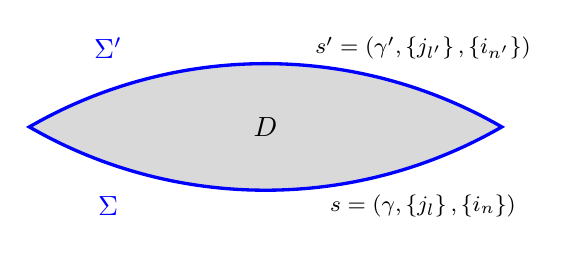
\begin{tikzpicture}
					\draw[very thick,blue,fill=gray,fill opacity=0.3] (3,0) -- (3,0) arc (60:120:6) -- (-3,0) -- (-3,0) arc (240:300:6) -- cycle;
					% \draw[very thick,blue](-3,0) arc (240:300:6);
					\node (Sigma) at (-2,-1) {\color{blue} $\Sigma$};
					\node (Sigma') at (-2,1) {\color{blue} $\Sigma'$};
					\node (D) at (0,0) {$D$};
					\node (s) at (2,-1) {\footnotesize $s=\left(\gamma,\left\{ j_l \right\},\left\{ i_n \right\}\right)$};
					\node (s') at (2,1) {\footnotesize $s'=\left(\gamma',\left\{ j_{l'} \right\},\left\{ i_{n'} \right\}\right)$};
				\end{tikzpicture}
				\caption{夹在两片类空超曲面 $\Sigma,\Sigma'$ 间的区域 $D$}\label{pic-D}
			\end{figure}

		\section{相干态表示}

			上一节中得到的跃迁振幅,其边界态是用量子的 spin-network 表示的,但物理上考虑,边界应赋半经典态,即第\ref{chp-application}章第\ref{sec-coherent_states}节 中定义的 相干态。为此,先注意到当 $i_e$ 取 LS coherent intertwiner $i_e=i_e(\{\myvec{n}_{fe}\})$ 时,在 $\Delta_v$ 的边界上诱导一个 LS 态 $\psi_v$,有
			\begin{equation}
				\begin{split}
					\amplitude_v(j_f,\myvec{n}_{fe}) &= (f_\gamma \psi_v)(\II)\\
					&= \left( \prod_{e\in \partial v} \int_{\SL{2,\mathbb{C}}} \dd{g_{ve}} \right) Y_\beta \psi_v(\{g_{ev} g_{ve'}\})\\
					&= \left( \prod_{e\in \partial v} \int_{\SL{2,\mathbb{C}}} \dd{g_{ve}} \right) \prod_{(e,e')} \mel{j_f,\myvec{n}_{ef}}{Y_\beta^\dagger g_{ev} g_{ve'} Y_\beta}{j_f,\myvec{n}_{e'f}},
				\end{split}
			\end{equation}
			其中约定 $g_{ev} = g_{ve}^{-1}$,则对整个跃迁振幅,有
			\begin{equation}
				\begin{split}
					&W_{\complex{K}^*}\left(\left\{ j_l\right\},\left\{ \myvec{n}_{ln} \right\}\right)\\
					={}& \sum_{\left\{ j_f \right\}} \prod_{f\in \complex{K}^*} \left( 2j_f + 1 \right) \prod_{\substack{(v,e)\\v\in e}} \int_{\SL{2,\mathbb{C}}} \dd{g}_{ve} \prod_{\substack{(e,f)\\e\in f}} \int_{S^2} \dd{\myvec{n}_{ef}} \prod_{v\in f} \mel{j_f,\myvec{n}_{ef}}{Y_\beta^\dagger g_{ev} g_{ve'} Y_\beta}{j_f,\myvec{n}_{e'f}},
				\end{split}
			\end{equation}
			这就是 spinfoam 跃迁振幅的 LS 相干态表示。使用全纯相干态表示更合适,因为全纯相干态是在经典态周围的高斯波包,但稍复杂一些,结果是\cite{Bianchi2010}
			\begin{equation}
				\begin{split}
					&\amplitude_v(\{H_f,t_f\})\\
					={}& \prod_{e\in \partial v} \int_{\SL{2,\mathbb{C}}} \dd{g}_{ve} \prod_{(e,e')} \sum_{j_f} \left( 2 j_f + 1 \right) \e{-j_f(j_f+1) t_f} \tr(D^{j_f}(H_f) Y_\beta^\dagger D^{(\beta (j_f+1),j_f)}(g_{ev}g_{ve'}) Y_\beta),
				\end{split}
			\end{equation}
			其中 $D^{j}$ 是 $\SU{2}$ 上的 Wigner D矩阵在 $\SL{2,\mathbb{C}}$ 上的解析延拓。

			\nomenclature{$D^j,\tensor{D}{^j_m_n}$}{Wigner D矩阵}

		\section{半经典极限与离散几何}

			spinfoam 跃迁振幅可定义两种极限,一是~\eqref{eq-continuous_limit} 中的连续极限,二是半经典极限,如图~\ref{pic-semiclassical_limit} 所示。半经典极限对应 $\hbar\rightarrow 0$,或量子数趋于无穷。故在 spinfoam 引力中,认为半经典极限为 $j_f \rightarrow \infty$。
			\begin{figure}[htbp!]
				\centering\small
				\begin{tikzpicture}
					\node (s) at (0,0) {spinfoam 引力};
					\node (R) at (5,0) {Regge 几何};
					\node (Q) at (0,3) {完整的量子引力};
					\node (c) at (5,3) {广义相对论};
					\draw[\myarrow] (s) -- node[above]{\scriptsize 半经典极限} (R);
					\draw[\myarrow] (s) -- node[left]{\scriptsize 连续极限} (Q);
					\draw[\myarrow] (Q) -- node[above]{\scriptsize 半经典极限} (c);
					\draw[\myarrow] (R) -- node[left]{\scriptsize 连续极限} (c);
				\end{tikzpicture}
				\caption{连续极限与半经典极限}\label{pic-semiclassical_limit}
			\end{figure}

			在 \cite{Barrett2009} 中研究了单个4-单形 $\Delta_v$ 的顶点振幅 $\amplitude_v(j_l,\myvec{n}_{ln})$,结果表明,若令 $j_f \mapsto \lambda j_f$,在 $\lambda\rightarrow \infty$ 极限下,注意到根据面积算符的谱,有 $A_l \simeq \gkappa \beta j_f$,则 $\gkappa \beta j_l \myvec{n}_{ln}$ 可视为 $\Delta_v$ 边界上的四面体各面的法矢,据此计算\emph{不足角}(deficit angle) $\theta_l$,则有渐进表达式
			\begin{equation}
				\amplitude_v \simeq \frac{1}{\mathcal{N}\lambda^{12}} \e{\ii \lambda S} + \text{c.c.},
			\end{equation}
			其中 $\mathcal{N}$ 是一个系数,
			\begin{equation}
				S = \sum_{l\in \gamma_v} \beta j_l \theta_l \simeq \frac{1}{\gkappa} \sum_{l\in\gamma_v} A_l \theta_l
			\end{equation}
			渐进为 Regge 作用量。故单个4-单形的半经典极限是正确的。

			韩慕辛和张鸣一于2011年对欧式号差\cite{Han2011rf}和洛伦兹号差\cite{Han2011re}的情况分别得到了更进一步的结果,对于任意的单复形 $\complex{K}$,令 $j_f \mapsto \lambda j_f$,则 $W_{\complex{K}^*}$ 具有 $\int \dd{x} a(x) \e{\lambda S(x)}$ 的形式,$S$ 称为“spinfoam 作用量”,$x$ 代表 spinfoam 变量。对于 $\lambda \rightarrow \infty$ 极限,它渐进为 $a(x_c) \e{\lambda S(x_c)}$,其中 $x_c$ 是 $S$ 的临界点(critical point),即
			\begin{equation}
				S'(x_c) =0 \qc \text{且} \Re S(x_c) = 0,
			\end{equation}
			对 spinfoam 作用量求解临界点,结果表明,除了用 $\myvec{n}_{ef}$ 可构造各个与 $e$ 对偶的四面体 $t_e$ 的法矢$N_{ef}$外,还有相邻四面体$t_e,t_{e'}$ 的公共面 $t_f$ 处满足 $N_{ef} = N_{e'f}$,故四面体具有正确的粘合。最后,spinfoam 作用量在临界点处也具有 Regge 作用量的形式。故至此可以说 spinfoam 引力的半经典极限是 Regge 作用量,而Regge 作用量取经典极限即为广义相对论的 爱因斯坦希尔伯特作用量。
